\newpage
\section{Test 5}
\label{Sec:test_5}

In the fifth test setting the rover is posed on and inclined plane.
Inclination angle of the slope has been set to 10$^\circ$. After the 10$^{th}$ second of simulation a simple PD controller
is set using position and velocity of the center of mass, in order to stop the rover on the slope. Rover stops effectively at $t = 25s$. 
Friction coefficient has been set to 0.8. Restitution coefficients (tangential and normal) have been set to zero. 

\begin{figure}[H]
  \centering
    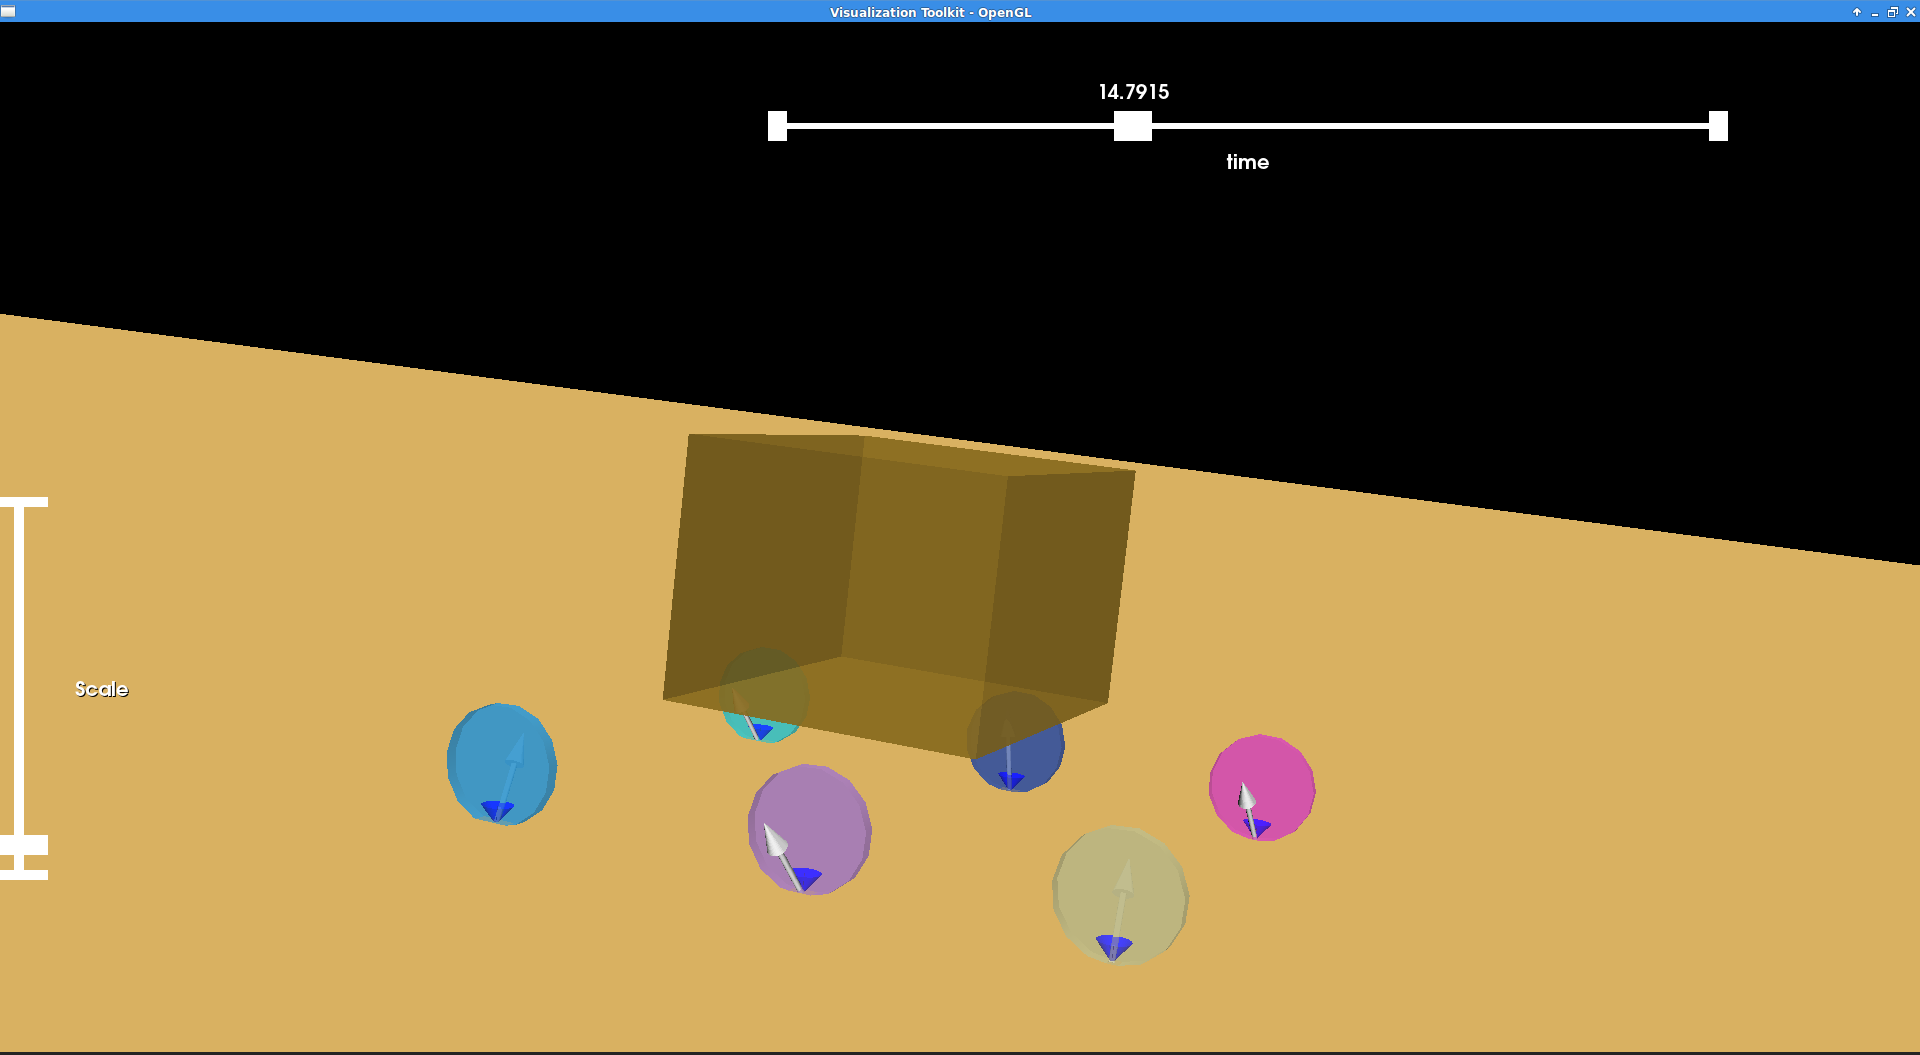
\includegraphics[width=0.8\textwidth]{run_5}
  \caption{Fifth test scenario}
\end{figure}

\noindent In this setting we are mostly interested in two phases:

\begin{enumerate} 
  \item $0s < t_s < 10s$
  \item $10s < t_s < 40s$
\end{enumerate}

\noindent In this case, following essential quantities have been plotted:

\begin{figure}[H]
  \centering
    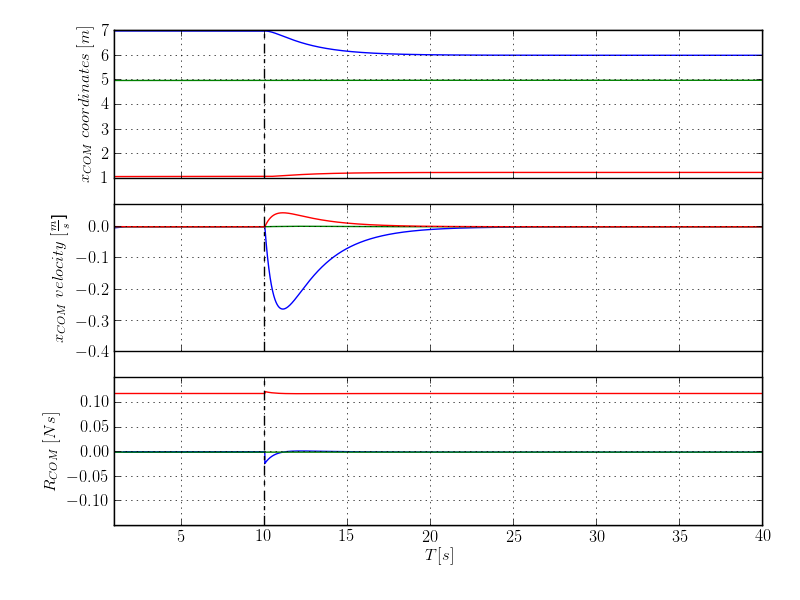
\includegraphics[width=0.8\textwidth]{xvpCOM5}
  \caption{position, velocity and reaction force of the mass center}
\end{figure}

\noindent \textbf{\textit{\Large{Comments}}}\\[1mm]
\noindent One can clearly see two phases of motion of the rover. In the end of the second phase rover stops its motion on the inclined plane which once again
demonstrates the efficiency of the nonsmooth friction-contact law. This can be seen in the figure 23 where in the second phase velocity components converge towards zero. 
This effect corresponding to a true nature of friction and can be captured in numerical experiments using nonsmooth laws. Using regularized laws to describe friction would not allow the system to retain non-zero torques with zero velocity.\\

\noindent Following additional quantities have been plotted:

\begin{figure}[H]
  \centering
    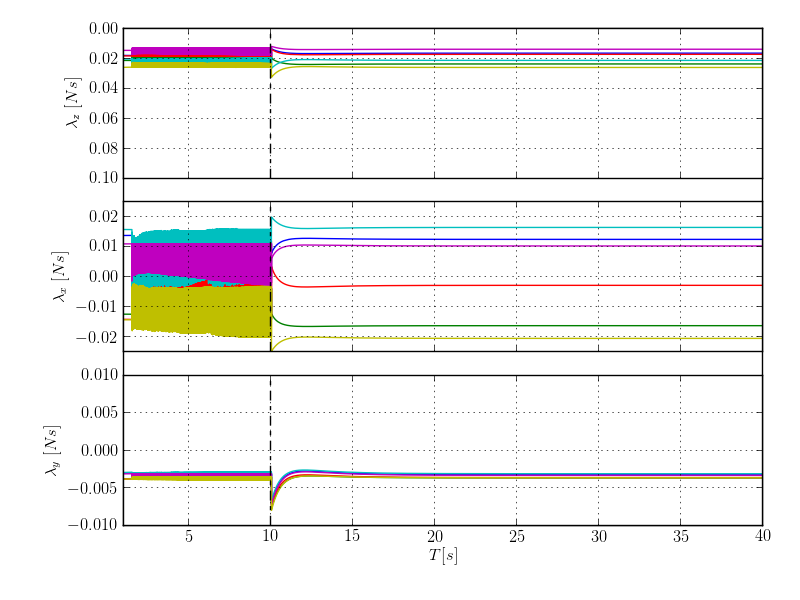
\includegraphics[width=0.8\textwidth]{lambdaNTS5}
  \caption{$\lambda_{N}$ - normal component of the contact force (impulsion) for each wheel}
\end{figure}

\begin{figure}[H]
  \centering
    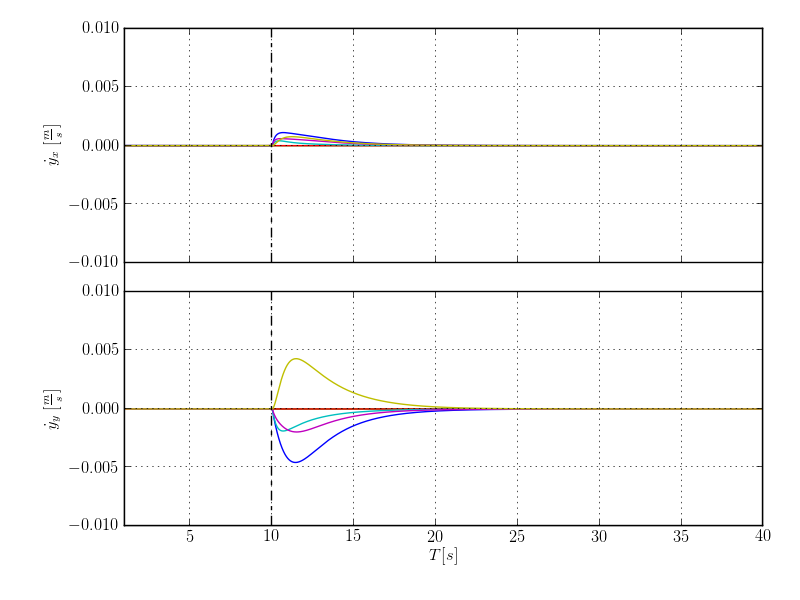
\includegraphics[width=0.8\textwidth]{yTxdotyTzdot5}
  \caption{$\dot{y}_{T_z}$ - tangential component z of the local contact velocity for each wheel}
\end{figure}

\noindent \textbf{\textit{\Large{Comments}}}\\[1mm]
\noindent As in the previous test setting, an immediate observation comes into mind as to the oscillations in the figure 24. Indeed, it is the same reason as previously that they appear in the plot.\\

